\documentclass[12pt, titlepage]{article}

\usepackage{booktabs}
\usepackage{tabularx}
\usepackage{longtable}
\usepackage{hyperref}
\usepackage{graphicx}
\usepackage{float}
\hypersetup{
    colorlinks,
    citecolor=black,
    filecolor=black,
    linkcolor=red,
    urlcolor=blue
}
\usepackage[round]{natbib}

\input{../Comments}
\input{../Common}

\newcounter{mnum}
\newcommand{\mthemnum}{M\themnum}
\newcommand{\mref}[1]{M\ref{#1}}

\begin{document}

\title{Verification and Validation Report: \progname} 
\author{\authname}
\date{\today}
	
\maketitle

\pagenumbering{roman}

\section{Revision History}

\begin{tabularx}{\textwidth}{p{3cm}p{2cm}X}
\toprule {\bf Date} & {\bf Version} & {\bf Notes}\\
\midrule
Mar. 3, 2025 & 1.0 & TA Feedback\\
Mar. 10, 2025 & 1.1 & Prior to Rev1\\
Mar. 3, 2025 & 1.0 & TA Feedback\\
Mar. 10, 2025 & 1.1 & Prior to Rev1\\
\bottomrule
\end{tabularx}

~\newpage

\section{Symbols, Abbreviations and Acronyms}

\renewcommand{\arraystretch}{1.2}
\begin{tabular}{l l} 
  \toprule		
  \textbf{symbol} & \textbf{description}\\
  \midrule 
  T & Test\\
  SRS & Software Requirements Specification\\
  M & Module \\
  \bottomrule
\end{tabular}\\

% \wss{symbols, abbreviations or acronyms -- you can reference the SRS tables if needed}

\newpage

\tableofcontents

\listoftables %if appropriate

\listoffigures %if appropriate

\newpage

\pagenumbering{arabic}

This document showcases the evaluation of the tests from the VnV plan for \progname.
The tests are categorized into functional and nonfunctional requirements that can be
seen in more detail in the VnV plan.

\section{Functional Requirements Evaluation}


\begin{longtable}{|c|c|p{8cm}|}
  \hline
  \textbf{Test Name} & \textbf{Result} & \textbf{Analysis}\\
  \hline
  \multicolumn{3}{|c|}{\textbf{Scheduling}}\\
  \hline
  test-FR8 & Passed & System can take availabilty data when creating team
  account.\\
  % \hline
  % test-FR9 & Passed & Covered by unit tests.\\
  \hline
  test-FR10 & Passed & Reschedule requests are able to be sent.\\
  \hline
  test-FR11 & Passed & Reschedule requests can be accepted and update the
  database accordingly.\\
  \hline
  test-FR12 & Failed & Feature must be added to notify team account users
  when their requests have been accepted.\\
  \hline
  test-FR18 & Failed & Score data currently does not update when using admin
  features.\\
  \hline
  test-FR20 & Passed & Schedule data is displayed if it exists in the
  database.\\
  \hline
  test-FR21 & Passed & Team only schedule data is displayed if it exists in
  the database.\\
  % \hline
  % test-FR22 & Passed & This feature is no longer planned for.\\
  \hline
  \multicolumn{3}{|c|}{\textbf{Accounts}} \\
  \hline
  test-FR1-1 & Passed & Season schedule is displayed to all users of all account types.\\
  \hline
  test-FR1-2 & Passed & Season standings is displayed to all users of all account types.\\
  \hline
  test-FR3-1 & Passed & Accounts are created and added to the system with the corresponding valid information.\\
  \hline
  test-FR3-2 & Passed & Accounts are not created or added to the system with invalid data.\\
  \hline
  test-FR4 & Failed & Feature must be added to change users' account details.\\
  \hline
  test-FR5-1 & Failed & Feature must be added for a user to delete their account once account credentials have been entered.\\
  \hline
  test-FR5-2 & Passed & Feature must be added for a user to delete their account once account credentials have been entered.\\
  \hline
  test-FR16-1 & Passed & Login succeeds for multiple accounts of varying credentials and account types given correct credentials for that account.\\
  \hline
  test-FR16-2 & Passed & Login fails for multiple accounts of varying credentials and account types given credentials that do not exist in the system.\\
  \hline
  %test-FR19 & Failed & \\ % this feature doesn't exist yet nor may the future implementation take the form of what is described in the SRS
  %\hline
  \multicolumn{3}{|c|}{\textbf{Team Structure}} \\
  \hline
  %test-FR2-1 & Passed & \\ % this feature doesn't exist yet nor may the future implementation take the form of what is described in the SRS
  %\hline
  %test-FR2-2 & Passed & \\
  %\hline
  %test-FR7 & Passed & \\
  %\hline
  %test-FR13-1 & Passed & \\
  %\hline
  %test-FR13-2 & Passed & \\
  %\hline
  test-FR15 & Failed & Feature must be added for a player level account user to join a team.\\
  %\hline
  %test-FR23 & Passed & \\ this feature doesn't apply anymore as captain accounts have been replaced with team accounts
  % \hline
  % \multicolumn{3}{|c|}{\textbf{Scoring/Standings}} \\
  % \hline
  % test-FR14-1 & Passed & \\
  % \hline
  % test-FR14-2 & Passed & \\
  % \hline
  % test-FR14-3 & Passed & \\
  % \hline
  % \multicolumn{3}{|c|}{\textbf{Alerts}} \\
  % \hline
  % test-FR6-1 & Passed & \\
  % \hline
  % test-FR6-2 & Passed & \\
  \hline
  \caption{Functional Requirements Test Results}
\end{longtable}
% \caption{Functional Requirements Test Results}


\section{Nonfunctional Requirements Evaluation}

\subsection{Usability}

Sandlot's Usability Survey Link used for testing: \href{https://forms.office.com/Pages/ResponsePage.aspx?id=B2M3RCm0rUKMJSjNSW9HcodvkeIlB8lOjrmyIWuVT7dUQ0hBNFRVTjFHWVhITDIzSklZRDRYTVZRMi4u}{Sandlot Usability Survey}

\begin{enumerate}
  \item{Readability: test-AP3, STY1, UP1\\}
  Brief Description(How tests were performed): The user was provided the website and asked
  to read groups of text or images such as the schedule or account registration fields.
  They would then be provided the survey form, provided above, to fill out and provide their own feedback
  on their experience. \\
  Average Result: Yes, the system was accessible. (3)\\
  Evaluation: After the tester(s) had read the Sandlot website's different texts and images,
  they found the website's readability to be up to a high quality, following a consistent
  stylistic formatting as evaluated from the resulting rating metric. This indicates that the
  text and images on the website are clear and easy to understand, which is crucial for user
  engagement and satisfaction. However, there is still room for improvement in ensuring that
  all text elements are uniformly accessible across different devices and screen sizes.
  \item{Registration/Login: test-EU2\\}
  Brief Description(How test was performed): The user was asked to register and sign in to
  an account they had created, identifying any faults such as login failure, incorrect
  password verification, etc., throughout their experience. They would then be provided the survey form, provided above, to fill
  out and provide their own feedback on their experience. \\
  Average Result: Strongly Agree (5)\\
  Evaluation: After the tester(s) had registered and signed in to the account they had
  created on the Sandlot website, they had found the website's registration and sign in process
  to function appropriately (i.e. providing correct sign in feedback if their password was
  incorrect) based on the received resulting rating metric. This high satisfaction score indicates
  that the registration and login processes are user-friendly and reliable. However, implementing
  additional security measures such as two-factor authentication could further enhance user trust
  and security. Features such as password strength checking and email confirmations would be
  beneficial to add on top of the current implementation.
  \item{Navigation: test-AP4, EU1, LR3\\}
  Brief Description(How tests were performed): The user was provided the website and asked
  to navigate to certain functionalities/pages such as viewing the schedule (EU1, LR3),
  rescheduling a game, etc. They would then be provided the survey form, provided above, to fill
  out and provide their own feedback on their experience. \\
  Average Result: Very/Somewhat Easy (4.4)\\
  Evaluation: After the tester(s) had navigated the Sandlot website's different pages
  (Schedule, Home, Profile, etc.), they found the website's navigation including
  its menus and links to be easily accessible and straightforward from the resulting
  rating metric. This high ease-of-use score suggests that the website's navigation is intuitive
  and user-friendly. However, further improvements could be made by adding more contextual help
  and tooltips to guide users through complex tasks.
\end{enumerate}

\begin{figure}[H]
\centering
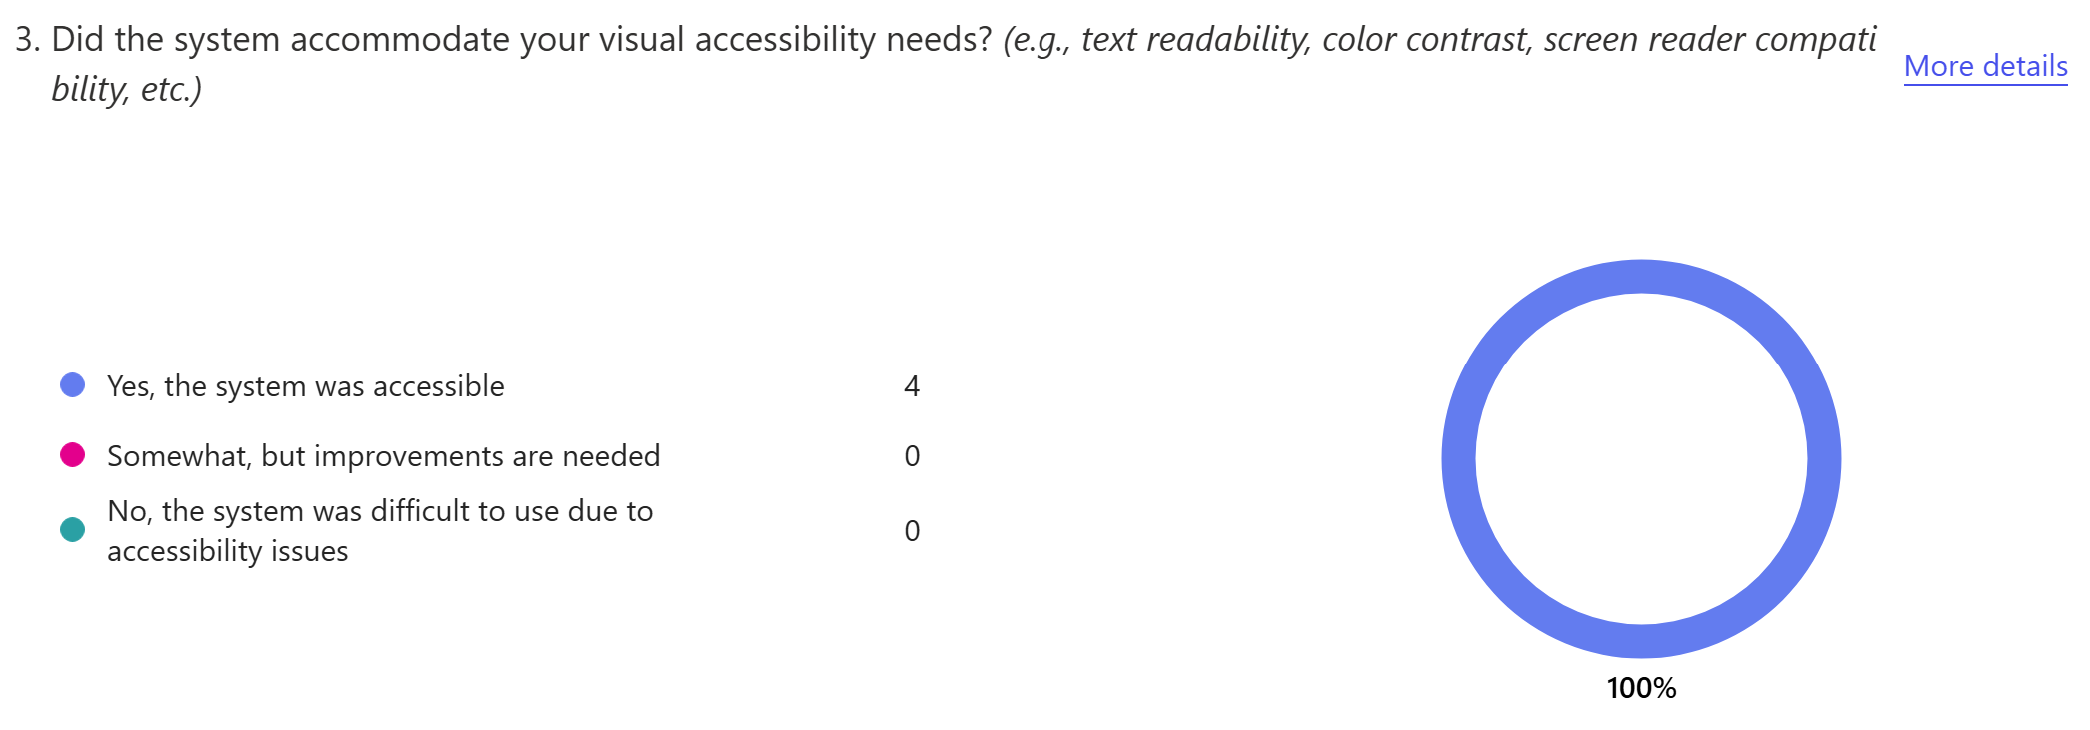
\includegraphics[scale=0.6]{survey_responses_visual.png}
\caption{Readability Response Metrics}
\label{visual}
\end{figure}

\begin{figure}[H]
\centering
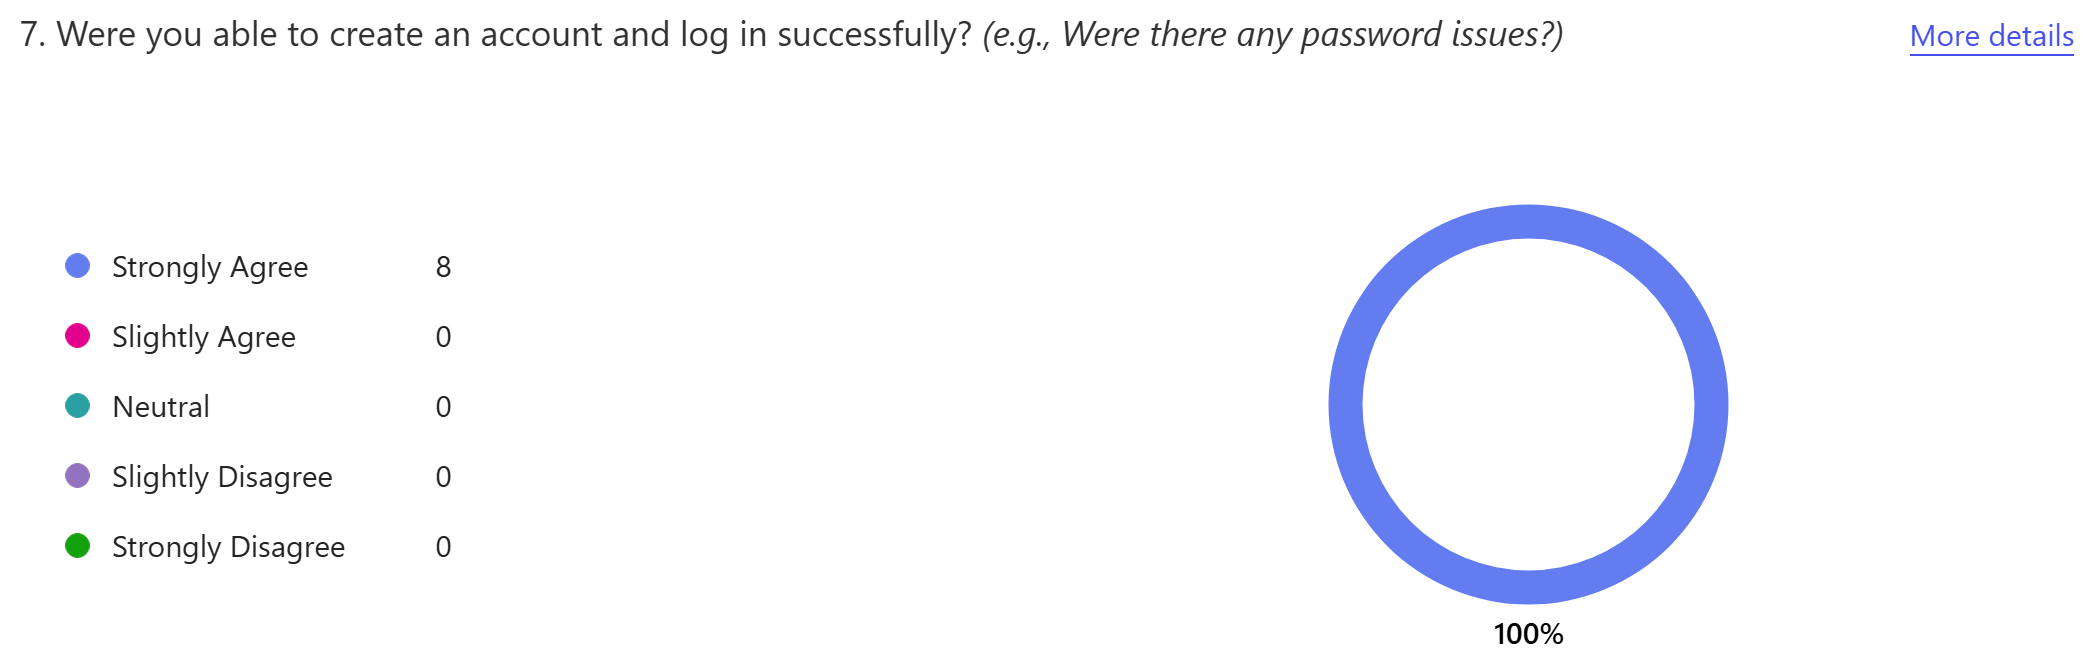
\includegraphics[scale=0.6]{survey_responses_register_signin.png}
\caption{Registration/Login Response Metrics}
\label{account}
\end{figure}

\begin{figure}[H]
\centering
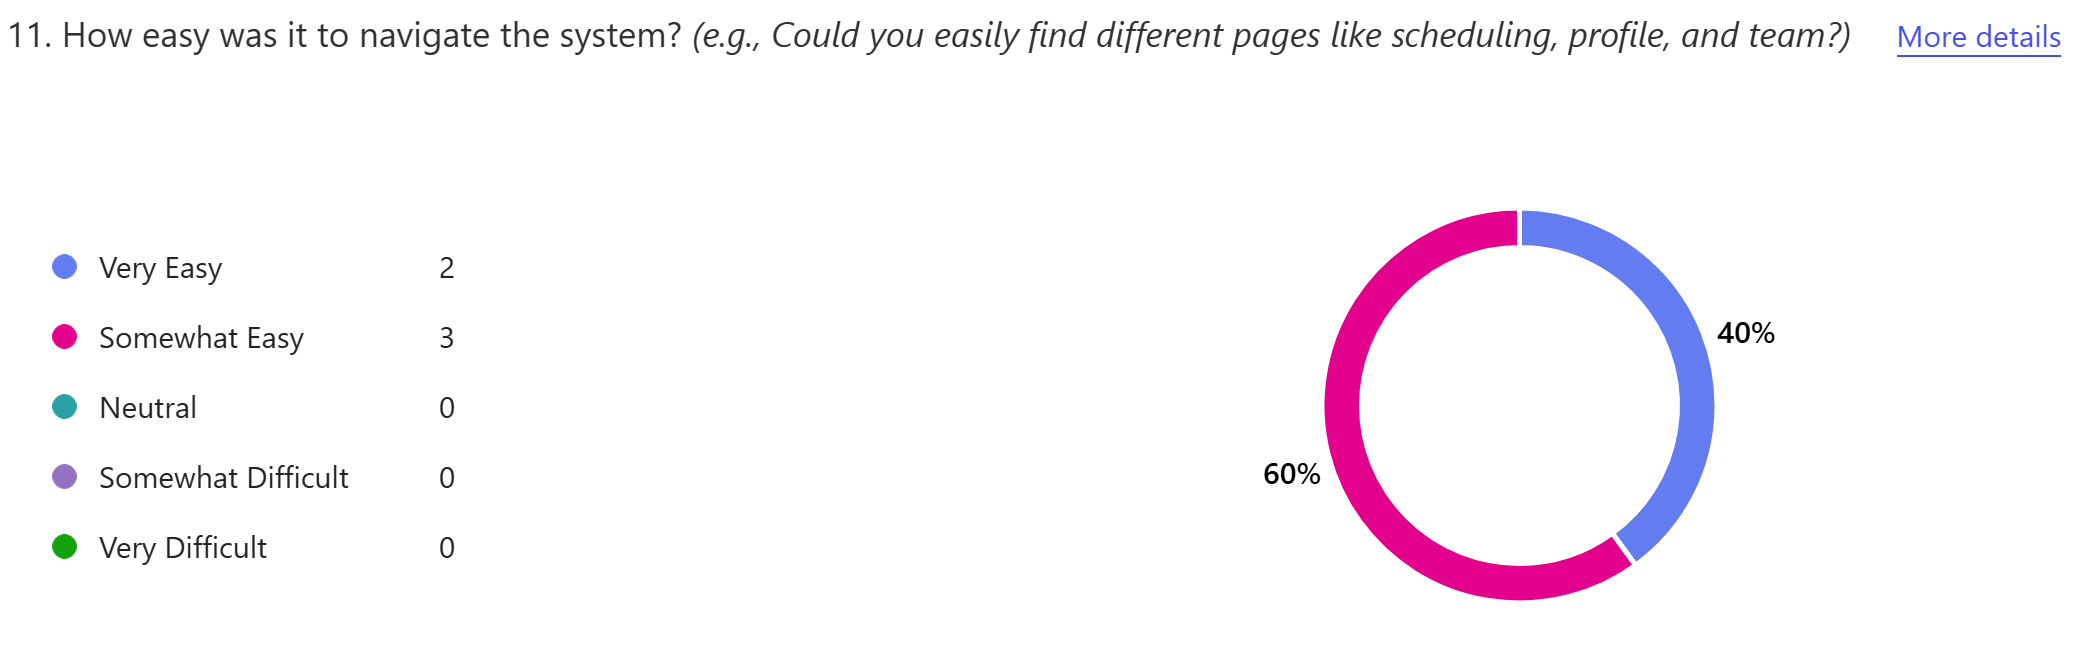
\includegraphics[scale=0.6]{survey_responses_navigation.png}
\caption{Navigation Response Metrics}
\label{nav}
\end{figure}
		
\subsection{Security}

\begin{enumerate}
  \item{General Access: test-AS1-1, AS1-2, PV1\\}
  Brief Description(How tests were performed): The tester was given general access to the
  website, in which they were not logged in to any account. They were then prompted to
  access both the season schedule (AS1-1) and standings (AS1-2), responding if each
  were both displayed correctly (i.e. all games showed up on the schedule, all teams
  showed up in the standings with their respective records). Also, the tester would attempt
  to locate sensitive information (PV1) (i.e. contact information of players) across the
  website and confirm if no such information was able to be observed. \\
  Average Result: Strongly/Slightly Agree (4.75)\\
  Evaluation: The tester(s) had successfully accessed the Sandlot website's season schedule and
  standings based on the resulting rating metric, without being logged in to an account. Additionally,
  they were not able to obtain contact information when browsing the website, securing sensitive
  information saved by the system from account users. The high rating score indicates that the
  website's general access is operating appropriately with little to no errors. However,
  improvements could be made to the loading times of the system as one comment made from the
  usability survey stated on initial loadings of a page, the initial time to view the page would
  take a little longer than expected.
  \item{Request Validation: test-AS6-1, AS6-2, IG1-2\\}
  Brief Description(How tests were performed): The tester was asked to sign in to a given
  account (player, team, commissioner), inputting valid (AS6-1) and invalid (AS6-2)
  account information. The system should then either log the tester into the account or
  deny their log in request due to invalid account information. When logged in with valid
  credentials, the tester should then submit a reschedule request (IG1-2) and accept/deny the
  request on the receiving end (the opposing team) by logging into their account. They will then
  confirm if the request had either been successfully denied or accepted. If the reschedule
  request was successfully accepted, the tester should confirm that the updated game day/time
  is reflected upon viewing the season schedule. \\
  Average Result: Slightly Agree (4)\\
  Evaluation: The tester(s) had successfully logged into their account with valid credentials
  and were denied access with invalid credentials based on the resulting rating metric. However,
  the reschedule request process was not as straightforward as expected, with some testers
  still being able to view their reschedule request even after they accepted or denied it.
  This indicates that the reschedule request process requires improvements to ensure that feedback
  is presented appropriately to users on their rescheduling actions (accept/deny). Moreover, the
  data gathered from the usability testing suggests that the system's account verification is
  secure, ensuring that only authorized users can access the system as well as their own personal
  information pertaining to their account.
  \item{Scheduling: test-IG1-1\\}
  Brief Description(How test was performed): The tester will be provided with sample
  scheduling data and be asked to generate a season schedule. This season schedule that is created
  should not have any conflicting scheduling conflicts that exist. \\
  Tests Conducted: 50\\
  Pass/Fail Rate: 43/50 (86\%)\\
  Evaluation: The tester(s) successfully generated a season schedule without any conflicting
  scheduling conflicts in 43 out of 50 attempts. The seven failures occured randomly and would
  be resolved when the website was reloaded. This high pass rate indicates that the scheduling algorithm
  is robust and reliable for most scenarios. However, improvements on the front end need to be
  investigated to ensure that all possible errors are resolved. These errors could occur from when the
  front end retrieves the scheduling data from the database or how it handles the data on the front end.
  The feedback from the usability testing also highlighted the need for better error messages and
  guidance in the display of the schedule, to help users understand and resolve issues more effectively.
\end{enumerate}

\begin{figure}[H]
\centering
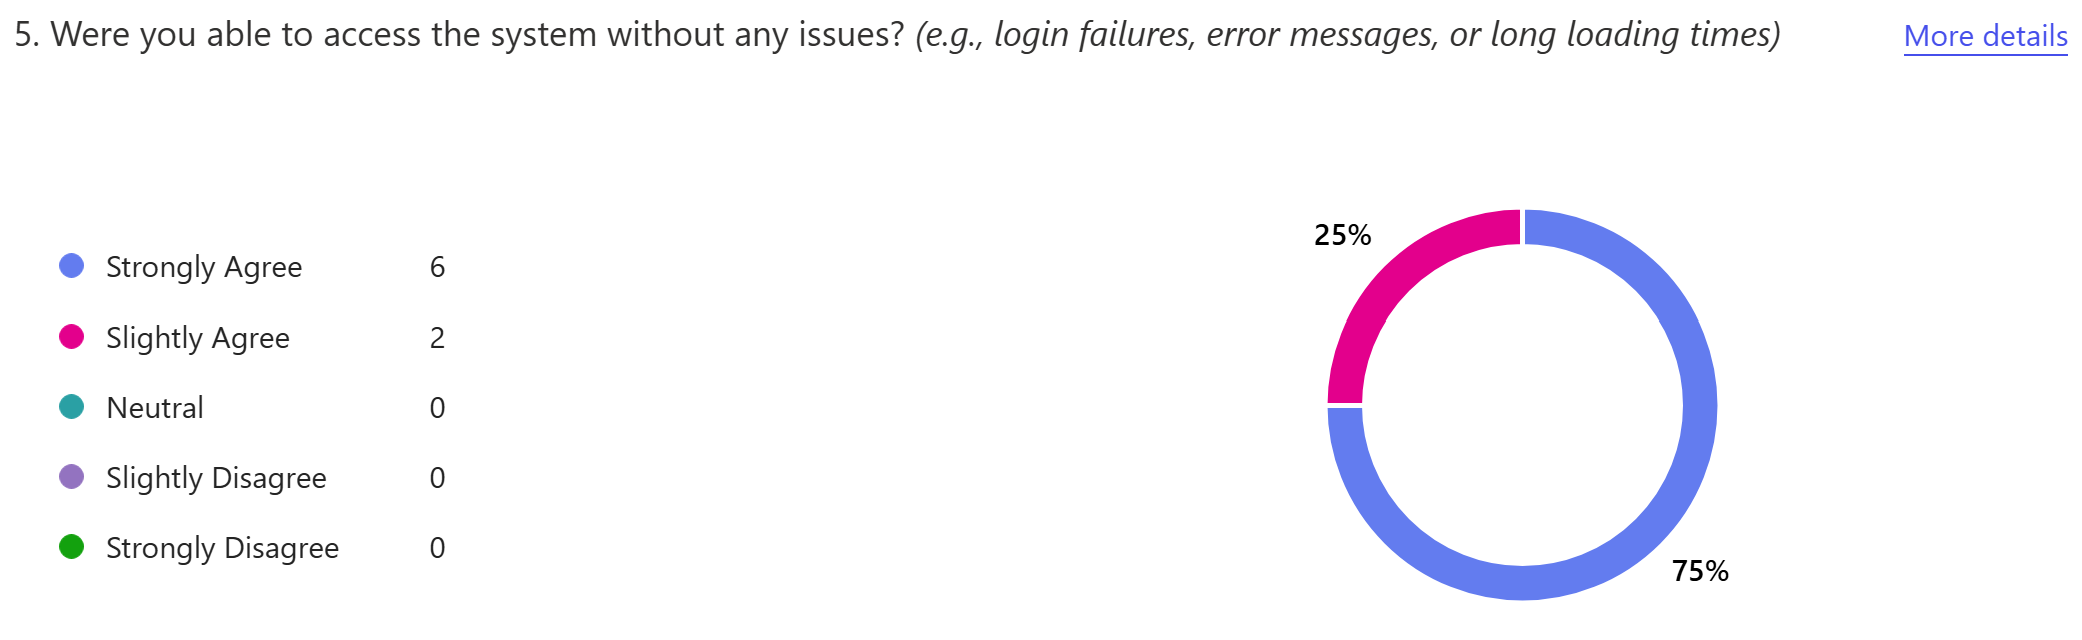
\includegraphics[scale=0.6]{survey_responses_access.png}
\caption{General Access Response Metrics}
\label{access}
\end{figure}

\begin{figure}[H]
\centering
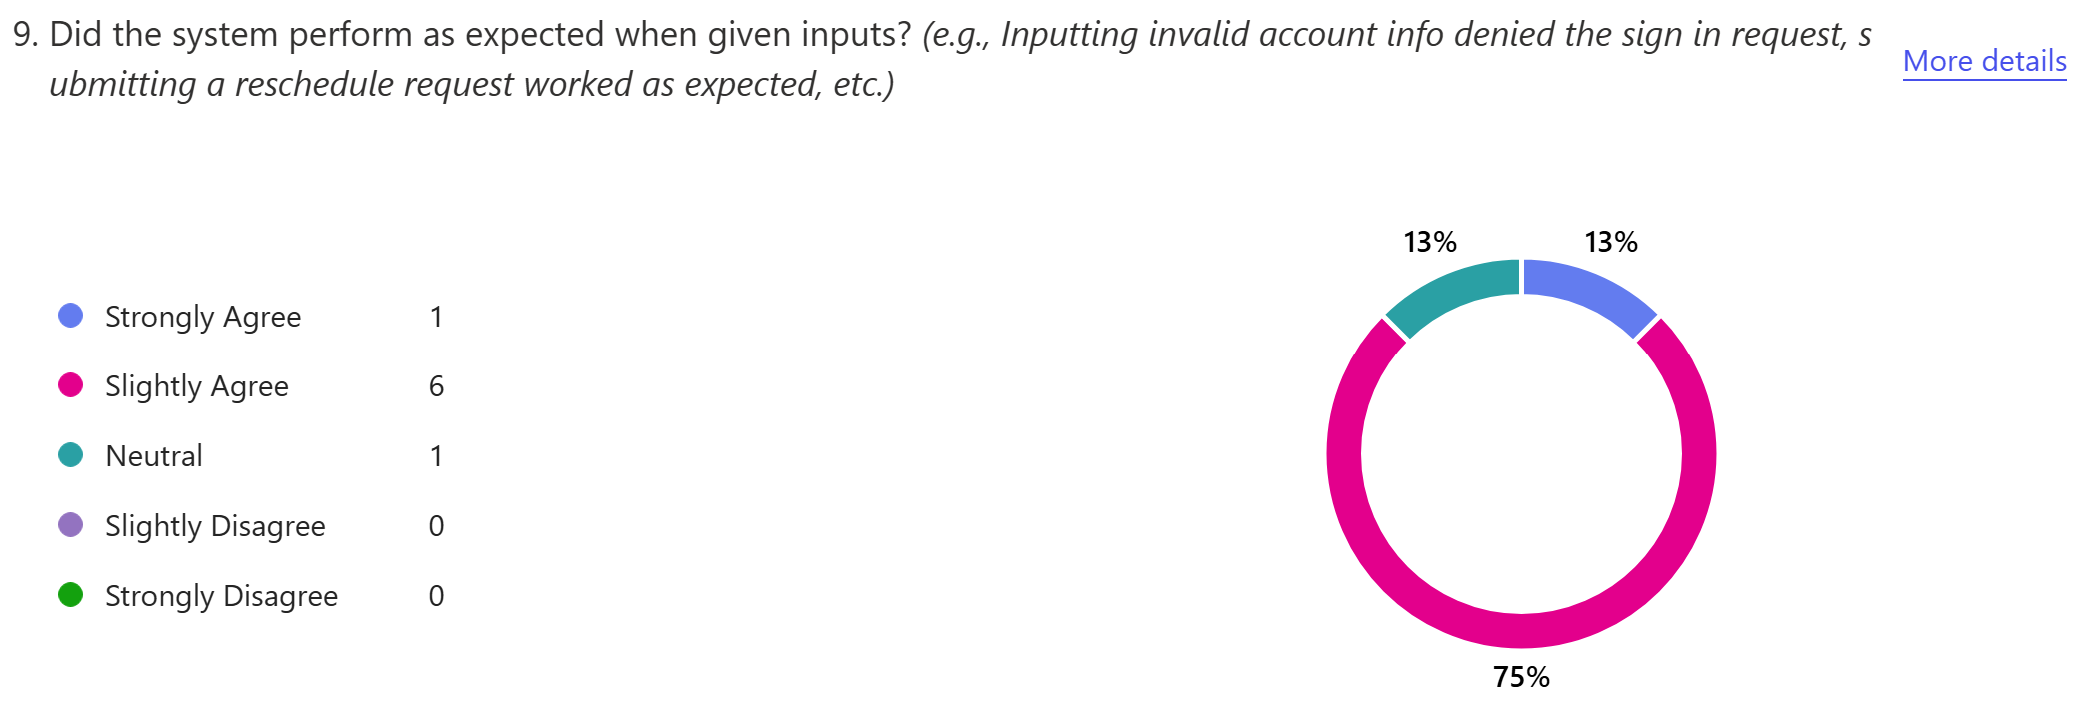
\includegraphics[scale=0.6]{survey_responses_validate_inputs.png}
\caption{Request Validation Response Metrics}
\label{validate}
\end{figure}
	
\section{Comparison to Existing Implementation}	

The current website used by the league, \href{https://www.gsasoftball.ca/}{GSA Softball},
provides basic functionalities for managing the McMaster Graduate Softball league, including
viewing schedules, team standings, weather information, etc. However, there are many links
or functionalities with the current website that are not operational, providing 404 Not Found errors.
The new Sandlot website introduces several improvements and additional features aimed at
enhancing the overall user experience and operational efficiency.

One of the significant improvements in the Sandlot website is the user interface design.
The new design provides a more modern and intuitive user experience, making it easier for
users of the system to navigate through different pages on the website. Additionally, the
layout is much cleaner, using a consistent stylistic formatting which enhances the readability
and accessibility of the system's text and images including the schedule, directory information
such as parking or weather information, and more. This is a notable improvement over the
existing website, which has a more dated and less user-friendly interface.

The Sandlot website also introduces advanced functionalities that are designed to streamline
league management and reduce the administrative burden on league organizers. For example, the
league organizers will be privy to multiple configuration options like division management and
general scheduling decisions such as a season's start and end date or minimum games played
by a team.

Another key enhancement is the integration of user accounts and personalized dashboards.
The Sandlot website allows players and captains to create accounts and access personalized
information relevant to their roles. This includes viewing their team's schedule and
managing player rosters. The current website lacks this level of personalization and
user-specific functionality.

In summary, the Sandlot website offers a comprehensive and user-friendly platform that
addresses many of the limitations of the current GSA Softball website. Improvements to the UI,
account management, and league configuration options provide a significant upgrade,
making the Sandlot website a more efficient and effective tool for managing league activities.

\section{Unit Testing}



\section{Changes Due to Testing}

% \wss{This section should highlight how feedback from the users and from 
% the supervisor (when one exists) shaped the final product.  In particular 
% the feedback from the Rev 0 demo to the supervisor (or to potential users) 
% should be highlighted.}

\subsection{Feedback from Rev 0 demo}

\begin{itemize}
  \item \textbf{User Role Implementation:} The demo showcased the user role functionality. However,
  the commissioner role was not yet available. The requirements for the commissioner role, as
  outlined in the SRS, were implemented for accessing league configuration and management options and
  other admin-level functionalities including alerts and generating a season schedule.
  \item \textbf{Scheduling Algorithm:} The team developed their own algorithm for scheduling, which was
  deemed reasonable. Configuration options were added to make the software general enough for other
  users while satisfying the specific requirements for Dr. Nease. Default values were set to meet
  Dr. Nease's requirements.
  \item \textbf{Rescheduling Functionality:} The team verified that rescheduling can be done and that it
  is straightforward. Additional features were added to enhance the rescheduling process, such as
  providing clear messages when a game cannot be rescheduled and explaining how the reschedule
  request works.
  \item \textbf{Usability Testing:} Usability testing was emphasized as very important for the
  project. The team conducted extensive usability tests and made several improvements based on the
  feedback received. This can be seen below in the user feedback section.
\end{itemize}

\subsection{Feedback from the Supervisor}

\begin{itemize}
  \item \textbf{Informataion Access:} Players can now see the email addresses of players on the same
  team but cannot access the email addresses of players on other teams' rosters. This ensures privacy
  while providing necessary contact information for a player's current team.
  \item \textbf{Team Schedule Location:} The team schedule is now prominently displayed on the
  schedule page, making it easily accessible to users. The entire season schedule is still available
  for view on the schedule page, if a user would like to access it.
  \item \textbf{Waiver Management:} The waiver process needs to be streamlined by integrating it into the
  website. Players should be able to view their signed waivers directly on the site, and a PDF version
  should be available for a player to download.
  \item \textbf{Join Request Limit:} The system should allow for configurable limits on the number of
  join requests a team can receive, providing flexibility for different league requirements.
  \item \textbf{Configuration Options:} Toggle options for reschedulability, adding fields and
  timeslots, choosing available days, and setting constraints should be implemented to make the system
  adaptable for other leagues.
  \item \textbf{Alerts/Announcements:} A bulk email feature needs to be added for sending alerts to specific
  groups of users. Announcements should be be dated and include headers and content for better
  communication.
  \item \textbf{Team Page Improvements:} Pie charts for scores, upcoming games, and team profile
  pictures would be desireable bonus features to add that could enhance the team pages.
  \item \textbf{Captcha and Security:} Captcha is desired to prevent automated sign-ups and
  enhance security.
\end{itemize}

\subsection{User Feedback}

\begin{itemize}
  \item \textbf{UI \& Navigation:}
  \begin{itemize}
    \item The GitHub logo, Documentation, and Github links were removed and a login/signup button was
    added to all pages, providing enhanced clarity to the registration/sign in process.
    \item Notices should be added to inform users to join a team to view the schedule if they are not
    part of a team.
    \item Messages explaining why a game cannot be rescheduled should be added.
    \item A legend for field colors needs to be added to the schedule.
  \end{itemize}
  \item \textbf{Rescheduling:}
  \begin{itemize}
    \item The reschedule request process should be clarified with a popup or description on the page,
    indicating how the rescheduling of a game works.
    \item Already played games should be greyed out/removed on both the reschedule menu and the regular
    schedule menu.
    \item The proposed dates section of a received reschedule request should clearly indicate who the
    request is coming from as currently no team information is visible unless a user were to verify the
    game themselves by navigating to the schedule page.
    \item Dates in reschedule requests should be reformatted to be more readable
    (e.g., "Tuesday, June 14th").
  \end{itemize}
  \item \textbf{Registration/Login:}
  \begin{itemize}
    \item A notice encouraging users to join a team should be added after signing up as a player.
    \item Sign-up email confirmations should be implemented once an account has been successfully
    registered by the user.
    \item Password checking on sign-up submission should be considered to ensure password strength.
    \item Two-factor authentication was considered for sign-up.
  \end{itemize}
  \item \textbf{General Improvements:}
  \begin{itemize}
    \item Preferred division field on team sign-up can be explained better with a tooltip.
    \item Offdays that appear in the registration process should be only added to the preferred off-day
    list, if the admin had configured the league to be played on those days. Also, if the league were
    to be scheduled on only one day of the week, the off-day selection should be disabled.
    \item Multiple off-days being selected was considered.
    \item Registering a new account should automatically sign the user in to their created account.
    \item Reschedule options need to be made more obvious with a dotted border and lighter color.
    \item Game start times should be highlighted as more important than end times. Considered removing
    end times altogether.
    \item Different colors, along with a legend, should be used to highlight games in the reschedule
    menu based on their status.
  \end{itemize}
\end{itemize}

\section{Automated Testing}

Currently, unit tests for the database, season scheduler, and reschedule modules are 
automated and continuously integrated using github actions to execute them on every push
and pull reqeust to our main branch. This ensures our code is as robust as possible when 
pushing to production branches while also saving us the hassle of manually running the tests 
ourselves. In the future we plan to extend our automated testing environments to produce 
visual test reports  in the form of HTML documents after each execution as well as provide 
code coverage metrics to help bolster our testing data.
		
\section{Traceability between Requirements and Modules}
		
\begin{description}
  \item [\refstepcounter{mnum} \mthemnum \label{mHH}:] Hardware Hiding Module
  \item [\refstepcounter{mnum} \mthemnum \label{mAC}:] Account Module
  \item [\refstepcounter{mnum} \mthemnum \label{mPL}:] Player Module
  \item [\refstepcounter{mnum} \mthemnum \label{mTE}:] Team Module
  \item [\refstepcounter{mnum} \mthemnum \label{mCM}:] Commissioner Module
  \item [\refstepcounter{mnum} \mthemnum \label{mAS}:] Account Structure
  Module
  \item [\refstepcounter{mnum} \mthemnum \label{mTS}:] Team Structure Module
  \item [\refstepcounter{mnum} \mthemnum \label{mSS}:] Schedule Structure
  Module
  \item [\refstepcounter{mnum} \mthemnum \label{mST}:] Standings Structure
  Module
  \item [\refstepcounter{mnum} \mthemnum \label{mS}:] Season Scheduler Module
  \item [\refstepcounter{mnum} \mthemnum \label{mRE}:] Reschedule Module
  \item [\refstepcounter{mnum} \mthemnum \label{mAL}:] Alerts Module
  \item [\refstepcounter{mnum} \mthemnum \label{mDB}:] Database Module
\end{description}

\newpage

% the table should use mref, the requirements should be named, use something
% like fref
\begin{table}
\centering
\begin{tabular}{p{0.2\textwidth} p{0.6\textwidth}}
\toprule
\textbf{Req.} & \textbf{Modules}\\
\midrule
FR-1 & \mref{mST}, \mref{mS},\\
% FR-2 & \mref{mTE}, \mref{mDB}\\
FR-3 & \mref{mAC}, \mref{mAS}\\
FR-4 & \mref{mAC}, \mref{mAS}\\
FR-5 & \mref{mAC}, \mref{mAS}\\
% FR-6 & \mref{mCM}, \mref{mAL}\\
% FR-7 & \mref{mTE}, \mref{mCM}\\
FR-8 & \mref{mPL},\\
% FR-9 & \mref{mS}\\
FR-10 & \mref{mPL}, \mref{mRE}\\
FR-11 & \mref{mPL}, \mref{mRE}\\
FR-12 & \mref{mPL}, \mref{mRE}\\
% FR-13 & \mref{mPL}, \mref{mTE}\\
% FR-14 & \mref{mPL}, \mref{mTE}\\
FR-15 & \mref{mPL}, \mref{mTE}\\
FR-16 & \mref{mAC}\\
% FR-17 & \mref{mPL}, \mref{mTE}\\
FR-18 & \mref{mCM}, \mref{mS}\\
% FR-19 & \mref{mPL}, \mref{mCM}, \mref{mTS}\\
FR-20 & \mref{mSS}, \mref{mS}\\
FR-21 & \mref{mTS}, \mref{mSS}, \mref{mS}\\
% FR-22 & \mref{mCM}, \mref{mSS}, \mref{mS}\\
% FR-23 & \mref{mTS}\\
% FR-24 & \mref{mAC}, \mref{mWA}\\
\bottomrule
\end{tabular}
\caption{Trace Between Functional Requirements and Modules}
\label{TblRT}
\end{table}

%\section{Code Coverage Metrics}

\bibliographystyle{plainnat}
\bibliography{../../refs/References}

\newpage{}
\section*{Appendix --- Reflection}

The information in this section will be used to evaluate the team members on the
graduate attribute of Reflection.

\input{../Reflection.tex}

\begin{enumerate}
  \item What went well while writing this deliverable? 
  \item What pain points did you experience during this deliverable, and how
    did you resolve them?
  \item Which parts of this document stemmed from speaking to your client(s) or
  a proxy (e.g. your peers)? Which ones were not, and why?
  \item In what ways was the Verification and Validation (VnV) Plan different
  from the activities that were actually conducted for VnV?  If there were
  differences, what changes required the modification in the plan?  Why did
  these changes occur?  Would you be able to anticipate these changes in future
  projects?  If there weren't any differences, how was your team able to clearly
  predict a feasible amount of effort and the right tasks needed to build the
  evidence that demonstrates the required quality?  (It is expected that most
  teams will have had to deviate from their original VnV Plan.)
\end{enumerate}

\subsection*{Team Reflection}

  \begin{enumerate}
    \item Which parts of this document stemmed from speaking to your client(s) or
    a proxy (e.g. your peers)? Which ones were not, and why?\\

    The parts of this document that stemmed from speaking directly to clients or peers include
    the changes due to testing section that had condensed all of the feedback received from the
    Rev 0 demo, the supervisor, and selected users. Additionally, the usability testing conducted,
    along with the analysis of the data collected was gathered from speaking to client(s) or a proxy.
    The parts of the document that did not come from client(s) or a proxy was the unit testing as
    the team had written multiple sets of unit tests that were used to test certain functionalities
    of the system such as the scheduling algorithm. These were based on best practices and our team's
    internal discussions to ensure the robustness and successful operation of the system.\\
    
    \item In what ways was the Verification and Validation (VnV) Plan different
    from the activities that were actually conducted for VnV?  If there were
    differences, what changes required the modification in the plan?  Why did
    these changes occur?  Would you be able to anticipate these changes in future
    projects?  If there weren't any differences, how was your team able to clearly
    predict a feasible amount of effort and the right tasks needed to build the
    evidence that demonstrates the required quality?  (It is expected that most
    teams will have had to deviate from their original VnV Plan.)\\

    The VnV Plan was different and required several changes before conducting actual Verification
    and Validation for reasons including access to actual users of the system and the constant
    iteration that had occured from when the VnV Plan was first written.
    These changes occurred because real-world testing often uncovers issues that
    are not apparent during the planning phase. The iterative feedback from users
    and the supervisor helped us identify and address these issues, however this prompted changes
    needing to be made for the initially written VnV Plan. Specifically, some of these changes included
    reducing the amount of tests that would proceed through the VnV process or tests that the team
    had deemed unnecessary and thus removed. In future projects, we would anticipate such changes by
    incorporating more flexible and adaptive planning processes, allowing for iterative testing and
    feedback loops to refine the VnV activities continuously.
    Despite these deviations from the original plan, our team was able to predict a feasible amount of effort
    and the right tasks needed to build enough data for a proper analysis of the system.
    This was achieved through team alignment with the project's goals and requirements, ensuring
    the scope of the project was feasible for completion within the given time frame.

\end{enumerate}

\subsection*{Nicholas Fabugais-Inaba -- Reflection}

\begin{enumerate}
  \item What went well while writing this deliverable?\\\\
  The organization of each team member working on a particular section was something that went
  very well as part of this deliverable. This allowed us to fill out the various sections of this
  deliverable with a high level of detail as each person could focus on a section that they felt most
  comfortable in writing about. Additionally, with the sections completed, our team was able to communicate
  effectively and provide feedback on each other's sections, ensuring that the deliverable
  would be written up to all of our standards.
  \item What pain points did you experience during this deliverable, and how
  did you resolve them?\\\\
  When conducting the usability testing, it was difficult to get a large number of users to test the
  system and provide enough feedback for the team to conduct an extensive analysis. Although there
  was a limited amount of data collected, the team was still able to utilize the data and provide
  a proper analysis. This was done by identifying consistent themes in the users' feedback as this
  would let us know areas of the system that either provided a strong user experience or parts of
  the system that required improvement.
\end{enumerate}

\subsection*{Jung Woo Lee -- Reflection}

\begin{enumerate}
  \item What went well while writing this deliverable?\\\\
  Having the VnV Plan allowed this deliverable to be done smoothly as it mostly involved performing the required
  tests outline in that document. Moreover, the team was able to stay organized and work on this document 
  in a timely manner by divvying the sections and working simultaneously.\\
  \item What pain points did you experience during this deliverable, and how
  did you resolve them?\\\\
  The usability testing was a bit difficult to conduct as it was hard to get a diverse and more extensive
  set of users to test the system. But even with the limited number of testers, the team was still able to gain
  a large quanitity of feedback that was used to analyze the system. This was done by identifying consistent
  themes in the users' feedback as this would let us know areas of the system that either provided a strong user
  experience or parts of the system that required improvement. 

\end{document}